%
% This document contains the chapter about coaxial components.
%
% Copyright (C) 2006 Stefan Jahn <stefan@lkcc.org>
%
% Permission is granted to copy, distribute and/or modify this document
% under the terms of the GNU Free Documentation License, Version 1.1
% or any later version published by the Free Software Foundation.
%

\chapter{Coaxial components}
%\addcontentsline{toc}{chapter}{Coaxial components}

\section{Coaxial cable}
%\addcontentsline{toc}{section}{Coaxial cable}

\begin{figure}[ht]
\begin{center}
\psfrag{er}{$\mathrm{\varepsilon_r}$}
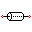
\includegraphics[width=0.35\linewidth]{coaxial}
\end{center}
\caption{coaxial line}
\label{fig:coaxial}
\end{figure}
\FloatBarrier

\subsection{Characteristic impedance}
%\addcontentsline{toc}{subsection}{Characteristic impedance}

The characteristic impedance of a coaxial line can be calculated as follows:
\begin{equation}
Z_0 = \dfrac{Z_{F0}}{2\pi\cdot\sqrt{\varepsilon_r}}\cdot\ln{\left(\dfrac{D}{d}\right)}
\end{equation}

\subsection{Losses}
%\addcontentsline{toc}{subsection}{Losses}

Overall losses in a coaxial cable consist of dielectric and conductor
losses.  The dielectric losses compute as follows:
\begin{equation}
\alpha_d = \dfrac{\pi}{c_0}\cdot f\cdot \sqrt{\varepsilon_r} \cdot \tan{\delta}
\end{equation}

The conductor (i.e. ohmic) losses are specified by
\begin{equation}
\alpha_c = \dfrac{1}{2}\cdot \sqrt{\varepsilon_r} \cdot\left(\dfrac{\dfrac{1}{D} + \dfrac{1}{d}}{\ln{\left(\dfrac{D}{d}\right)}}\right)\cdot\dfrac{R_S}{Z_{F0}}
\end{equation}

with $R_S$ denoting the sheet resistance of the conductor material,
i.e. the skin resistance
\begin{equation}
R_S = \sqrt{\pi\cdot f\cdot \mu_r \cdot \mu_o \cdot \rho}
\end{equation}

\subsection{Cutoff frequencies}
%\addcontentsline{toc}{subsection}{Cutoff frequencies}

In normal operation a signal wave passes through the coaxial line as a
TEM wave with no electrical or magnetic field component in the
direction of propagation.  Beyond a certain cutoff frequency
additional (unwanted) higher order modes are excited.
\begin{align}
f_{TE} &= \dfrac{c_0}{\pi\cdot\left(D + d\right)}
\;\;\;\;\rightarrow\;\;\;\; \textrm{TE(1,1) mode}\\
f_{TM} &= \dfrac{c_0}{2\cdot\left(D - d\right)}
\;\;\;\;\rightarrow\;\;\;\; \textrm{TM(n,1) mode}
\end{align}
